% To use the nomenclature: compile with makeindex %.nlo -s nomencl.ist -o %.nls in between pdflatex compilations

\documentclass[a4paper,12pt,oneside]{article}

% Packages

\usepackage[utf8]{inputenx}
\usepackage[english]{babel}

\usepackage[compact]{titlesec}
%%% Bug correcton of titlesec package to show section numbers:
\usepackage{etoolbox}
\makeatletter
\patchcmd{\ttlh@hang}{\parindent\z@}{\parindent\z@\leavevmode}{}{}
\patchcmd{\ttlh@hang}{\noindent}{}{}{}
\makeatother
%%%

\usepackage{graphicx}
\usepackage{amsmath,amssymb,mathrsfs}
\usepackage{fancyhdr}
\usepackage{calc}
\usepackage{titling}
\usepackage[T1]{fontenc}
\usepackage{mathtools}
\usepackage{mathptmx}

\usepackage[hyphens]{url}

\usepackage[none]{hyphenat}

\usepackage{amsfonts}
\usepackage{rotating}
\usepackage{graphicx}
\usepackage{epstopdf}
\usepackage{float}

\usepackage[a4paper]{geometry}

\usepackage[centerlast,small,sc,tableposition=top]{caption}
%\setlength{\captionmargin}{20pt}

\usepackage{hyperref}
   
\usepackage[style=numeric,backend=bibtex,bibencoding=ascii]{biblatex}
\usepackage{csquotes}

\usepackage{appendix}

\usepackage[usenames,dvipsnames]{xcolor} % Permite poner texto en color a traves de \textcolor{Color}{Texto}
\usepackage{pdfpages}
\usepackage{float}

\floatstyle{plaintop}
\restylefloat{table}
\usepackage{ltxtable}

\usepackage{siunitx}

\usepackage[titles]{tocloft}

\usepackage{listings}

\usepackage[intoc]{nomencl}
%=========================TAULES============================================================================================
% Es crea una nova comanda per insertar una taula. En aquest cas estara dintre de la carpeta taules. Per tal de fer servir la comanda \taula{Nom del fitxer}{amplada} on amplada pot ser \linewidth que es l'amplada de la linia, es pot posar 0.7\linewidth pq sigui un 70% de l'amplada.
\newcommand{\taula}[2]{\LTXtable{#2}{tables/#1}} 
%\renewcommand{\tablename}{Tabla} %per posar tabla al caption de les taules

%=========================INSERTAR IMATGES==================================================================================
%Aquesta macro inserta una imatge centrada. Per tal de colocar la imatge s'ha de fer servir la comanda:
%	\imatge{Nom fitxer dintre carpeta imatges}{Titol de la imatge}{Amplada}
%	el \label queda definit com el nom del fitxer
\newcommand{\imatge}[3]{
 \begin{figure}[htb]
  \begin{center}
   %\includegraphics[width=#3cm,angle=-90]{#1}
   \includegraphics[width=#3\linewidth]{#1}
   \caption{#2}
   \label{fig:#1}
  \end{center}
 \end{figure}
}

\newcommand{\imatgeR}[4]{
 \begin{figure}[htb]
  \begin{center}
   \includegraphics[width=#3\linewidth,angle=#4]{#1}
   \caption{#2}
   \label{fig:#1}
  \end{center}
 \end{figure}
}

\hypersetup{
    colorlinks,
    linkcolor={blue!80!black},
    citecolor={blue!80!black},
    urlcolor={blue!80!black}
}

% Espaiat a l'index
%\setlength{\cftbeforechapskip}{0.1ex} % Nomes al report i altres amb \chapter
\setlength{\cftbeforesecskip}{0.5ex}

% Portada

\newcommand{\authorname}{\textbf}
\newcommand{\authorgroup}{\emph}
\newcommand{\authoraddress}{\emph}
\newcommand{\authormail}{\emph}

\makeatletter
\def\@maketitle{%
  \newpage
  \null
%  \vskip 2em%
  \begin{center}%
  \let \footnote \thanks
    {\LARGE\MakeUppercase \@title \par}%
    \vskip 1.0em%
    {\Large\subject{}}
    \vskip 1.0em%
    {\normalsize
      \lineskip .5em%
      \begin{tabular}[t]{c}%
        \@author
      \end{tabular}\par}%
    \vskip -0.5em%  
    {\large\bf Group: \group{}}
    \vskip 1em%
%    \vfill
    {\large \@date, \city{}}%
  \end{center}%
  \par
  \vskip -0.5em}
\makeatother

%Maketitle Conf______________________________________________________
%\pretitle{\begin{center}\Large\MakeUppercase}
%\posttitle{\\\subject{}\end{center}}

%\preauthor{\begin{center}\normalsize \lineskip 0.5em\begin{tabular}[t]{c}}
%\postauthor{\end{tabular}\par\end{center}}

%\predate{\begin{center}\normalsize}
%\postdate{, \city{}\par\end{center}}
%_____________________________________________________________________


% Headers___________________________________________________________

\pagestyle{fancy}
\fancyhead[L]{\subject{}, ESEIAAT, Group \group{}}
\fancyhead[R]{\thedate{}, \city{}}

\setlength{\headheight}{15pt} 

%___________________________________________________________________

\DeclarePairedDelimiter{\norm}{\lVert}{\rVert}

\newcommand{\vnorm}[1]{\norm{\vec{#1}}}

\sloppy % better line breaks

\setlength{\nomitemsep}{-\parsep} % Nomenclature spacing

\newcommand{\fref}[1]{Fig.~\ref{#1}}
\newcommand{\tref}[1]{Tab.~(\ref{#1})}
\newcommand{\eref}[1]{Eq.~(\ref{#1})}
%\newcommand{\cref}[1]{Cap.~\ref{#1} \nameref{#1}} % \chapter references not available in article
\newcommand{\sref}[1]{Sec.~\ref{#1} \nameref{#1}}
\newcommand{\aref}[1]{Ap.~(\ref{#1})}
\newcommand{\alref}[1]{Algorithm~\ref{#1}}
\newcommand{\ejref}[1]{Ex.~(\ref{#1})}

\DeclareSIUnit\curie{Ci}

\graphicspath{{./images/}{./images/fix/}}

%\begin{figure}
%  \centering
%   \includegraphics[width=5cm]{shadow01}
%   \caption[Model UAV Shadow-MK1 a la EETAC.]{%
%    Model UAV Shadow-MK1 a la EETAC%
%    \footnotemark{}%
%   .}
%   \label{fig:shadow01}
%\end{figure}
%\footnotetext{Extret de: \url{http://eetac.upc.edu/ca/node/616}}

% ARTICLE DATA ENTRY_________________________________________________

% Title_______________________________________________________

\title{TITOL}

% Authors_____________________________________________________

\author{
	\authorname{Jordi Alcón Clemente}\\
	\authormail{\href{mailto:jordialconclemente@gmail.com}{jordialconclemente@gmail.com}}\\
	\authorname{Jordi Alcón Clemente}\\
	\authormail{\href{mailto:jordialconclemente@gmail.com}{jordialconclemente@gmail.com}}\\
% 	\authorgroup{Universitat Politècnica de Catalunya, BarcelonaTech (UPC)}\\
% 	\authorgroup{Escola Superior d’Enginyeries Industrial, Aeroespacial i Audiovisual de Terrassa}\\
% 	\authoraddress{Terrassa Campus, C. Colom, 1 08222 Terrassa. Telèfon 93 739 8102 / 93 739 8200.}\\
\\
}

\date{Mes 2018}

\newcommand{\city}{Terrassa}
\newcommand{\subject}{Assignatura}
\newcommand{\group}{01}


% Misc_____________________________________________________
%\renewcommand{\nomname}{List of Symbols}
\makenomenclature
 
\renewcommand{\nompreamble}{The next list describes the symbols used within the body of the document:}

\addbibresource{myrefs.bib}

% Article Body_____________________________________________

\begin{document}

\maketitle \thispagestyle{empty}

% Table Oof Contents________________________________________________
\noindent\makebox[\linewidth]{\rule{0.8\textwidth}{1pt}}
\newpage
\tableofcontents
\noindent\makebox[\linewidth]{\rule{0.8\textwidth}{1pt}}
\section*{About the project}
\addcontentsline{toc}{section}{About the project}

This project was theoretically supposed to be carried out by four people, but just two members of the group have made it.

Not a single meeting was held, as one of the members was 'never available'. He had a completely passive attitude towards this project, not caring about its completion. The only thing that he did was writing a couple of paragraphs in the last week before the deadline that were a whole bunch of nonsense, such as calculating the brake thrust $\Delta V_1$, which is given at the beginning in the definition of the problem.

The other member had a more positive attitude, but claiming a complete lack of understanding and complaining about a heavy workload due to other subjects, he didn't make anything until four days before the deadline. As they both had to work on the same part of the project, he was supposed to correct the mistakes of the first one. Two days before deadline the mistakes were still there. Those mistakes are not a consequence of the difficulty of the project, they are caused by a total lack of attention.   

For the reasons exposed, we consider that this project should not be taken into consideration in their final mark, as this rewards this kind of behavior towards teamwork ("let them work, I'll pass doing nothing"). All in all, it makes group work unfair and painful for the ones that really make it.
\newpage
\printnomenclature

% Input main content________________________________________

\nomenclature{$\Delta V$}{Velocity impulse}
\nomenclature{$H$}{Altitude}
\nomenclature{$d_{SJ}$}{Jupiter orbital radius}
\nomenclature{$d_{SE}$}{Earth orbital radius}
\nomenclature{$d_p$}{Periapsis radius}
\nomenclature{$d_a$}{Apoapsis radius}

% \section*{Foreword}
% \addcontentsline{file}{sec_unit}{entry}


\section{Problem definition}\label{sec:problem_definition}

A space vehicle has to be sent to Jupiter to perform some observations. This communication is aimed to describe the preliminary design of the trajectory in order to establish an initial $\Delta V$ budget for the mission. The proposed trajectory is to perform the escape from Earth and enter into an elliptical orbit around the Sun. This elliptical orbit is modified to encounter the Earth, where a natural gravity assist is performed. The gravity assist modifies the elliptical orbit around the Sun in order to intersect Jupiter's orbit. The study also considers another trajectory to compare with.

The study contains the following points:

\begin{enumerate}
\item An initial $\Delta V$ is applied to escape from the Earth and enter into an elliptical orbit around the Sun.

	\begin{enumerate}
	\item \label{it:escape_two_steps_jupiter} Calculation of the minimum $\Delta V_{e}$ needed to escape from Earth as a function of the parking orbit altitude $(H_0)$. Once in orbit around the Sun, a second $\Delta V_{1J}$ is calculated, which is applied to modify the orbit into an ellipse with its apoapsis equal to the radius of Jupiter's orbit.
	
	\item \label{it:escape_one_step_jupiter} Calculation of the minimum $\Delta V_{0J}$ needed to escape from Earth as a function of the parking orbit altitude $(H_0)$. Considering that the resulting elliptic orbit around the Sun has its apoapsis equal to the radius of Jupiter's orbit. This maneuver is performed in a single $\Delta V_{0J}$.
	
	\item Based on the results of the previous cases the optimum parking altitude is selected for each case and used in the rest of the study, where needed.
	\end{enumerate}

\item Design of the trajectory from Earth to Jupiter.

	\begin{enumerate}
	\item \label{it:direct} A direct transfer maneuver to reach Jupiter, including a $\Delta V_{i}$ to insert the vehicle at Jupiter's orbit at the same altitude than Europa, is studied. The total $\Delta V_T$ needed and the travel time to reach Jupiter are computed.

	\item \label{it:gravity_assist} Different trajectories with a single $\Delta V_{0}$ to escape from Earth, another $\Delta V_{1}$ to modify the trajectory to encounter Earth and perform the gravity assist, and a last $\Delta V_{i}$ to insert the vehicle at Jupiter's orbit at the same altitude than Europa are studied.
    
    For a $\Delta V_{0} = 4 \si{[km/s]}$ and $\Delta V_{1} = -650 \si{[m/s]}$ the following results are presented. \textit{Note: Use the angles solution of the smallest quadrant.}
    \begin{enumerate}
    \item Radius of apoapsis of the Jupiter's approach elliptic orbit as a function of the periapsis of the gravity assist.
    \item The heliocentric velocity of the vehicle after the gravity assist $(\vnorm{u_{v+}})$ as a function of the periapsis of the gravity assist.
    \item The velocity at the apoapsis of the Jupiter's approach elliptic orbit $(\vnorm{u_{a3}})$, as a function of the periapsis of the gravity assist.
    \item The total $\Delta V_T$ budget as a function of the periapsis of the gravity assist.
    \item The elliptical orbits and intersection points for a single value of the periapsis of the gravity assist are plotted, so a scale plot is provided.
    \end{enumerate}
    
    \item A study to minimize the $\Delta V_T$ budget for the trajectory with the gravity assist is conducted. The design variables are the two first $\Delta V$'s and the periapsis of the gravity assist. Explain the methodology used to perform the minimization and provide graphs to facilitate the comprehension of the results. \textit{Note: Be careful with solutions that are not physically possible, for example gravity assist trajectory entering the atmosphere.}
    
	\end{enumerate}

\item Schemes of the different orbits and trajectories are presented for all of the studied trajectories.

\item \textit{\textbf{As a bonus}, Compute the travel time form Earth to Jupiter for the trajectory \ref{it:gravity_assist} with a periapsis altitude for the gravity assist equal to $H_{\pi} = 450 \si{[km]}$. (Maximum 1 additional point)} \textbf{Hint: Search bibliography for mean anomaly and eccentric anomaly.}
\end{enumerate}




\section{Governing equations}\label{sec:governing_equations}

In this section the governing equations of the problem described in \sref{sec:problem_definition} are detailed.

\subsection{Hypothesis}

\begin{itemize}
\item All orbits are contained in the same plane.
\item Earth and Jupiter orbits are circular with radius $r_c$ defined as \eref{eq:radi_mig}.

\begin{equation}\label{eq:radi_mig}
d_c = \frac{d_a + d_p}{2}
\end{equation}

\item $\Delta V$ to escape from Earth is applied at a certain time which achieves that the initial velocity of the vehicle's orbit around the Sun is tangent to the Earth's orbit around the Sun.

\item Neglect the initial altitude when approaching and leaving a planet. Radius of sphere of influence $r_{SOI}$: $$r_{SOI} = 0 \si{[km]}$$
\end{itemize}

\subsection{Scape maneuver} \label{sec:scape_maneuver}

To begin the study an initial $\Delta V_{i}$ needed to scape the orbit of Earth and enter into an elliptical orbit around the Sun will be considered.

%%\subsubsection{Earth to Jupiter with two thrusts}\label{sec:two_thrusts}
\begin{figure}[H]
	\centering
		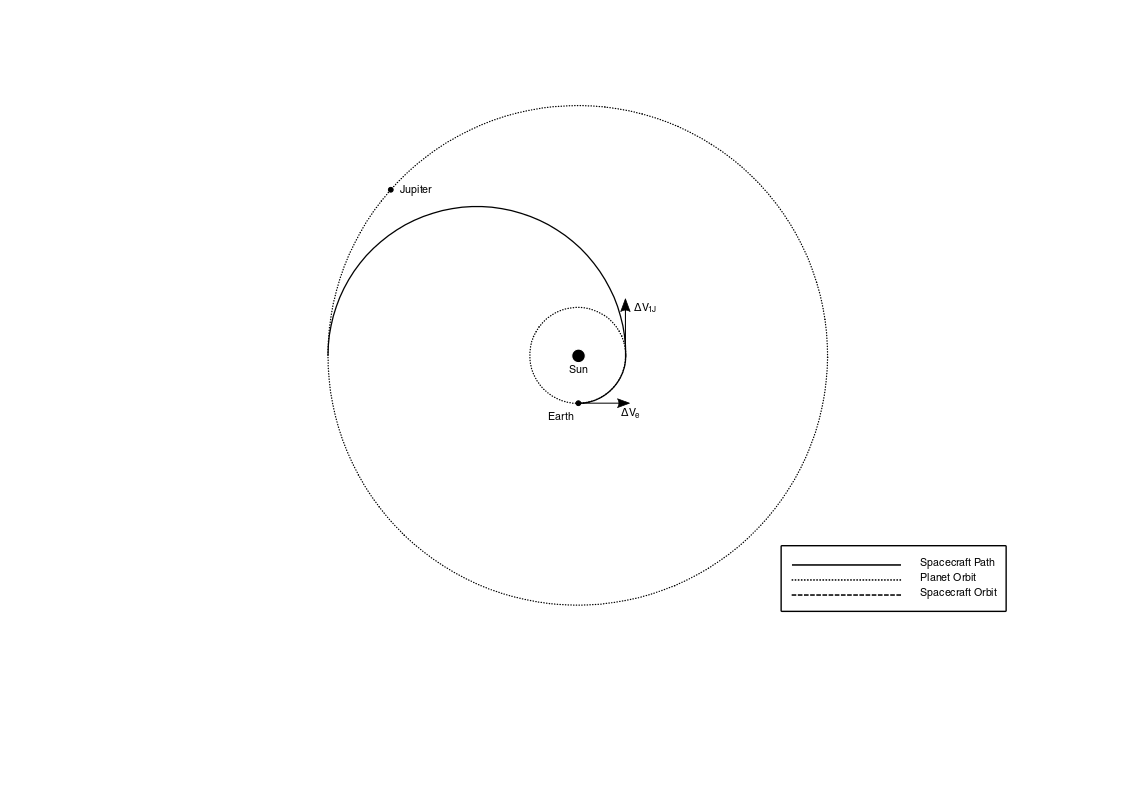
\includegraphics[width=\textwidth]{parabolica.png}
	\caption{Earth to Jupiter with two $\Delta V$}
	\label{fig:parabolica}
\end{figure}

The objective is to reach an elliptical orbit around the Sun whose apoapsis radius equals Jupiter's orbital radius. The starting point is  a satellite orbiting Earth at a determined $H_0$. In order to achieve this, two thrusts will be applied. 

\begin{itemize}
\item The first thrust will make the vehicle escape Earth's sphere of influence with a parabolic orbit. This can be calculated by substracting the speed of the satellite ($V_{s}$) from the Earth's scape velocity ($V_{e}$). To calculate $\Delta V_{e}$ it is imposed that the mechanical energy with respect to Earth equals zero at infinity.

\begin{equation}\label{eq:thrust}
\Delta V_e = V_e - V_s = \sqrt{\frac{2\mu_E}{R_E + H_0}}-\sqrt{\frac{\mu_E}{R_E+H_0}}
\end {equation}

After this first thrust, relative speed between Earth and the spacecraft will be zero, hence spacecraft's speed relative to the Sun will be the same as Earth's. Therefore, once this thrust has been applied, the vehicle will describe a circular orbit around the Sun whose radius will be equal to Earth's orbital radius. This thrust depends on initial $H_0$, as shown in . %%ref to figure 1 

\item A second thrust is used to bring the spacecraft to an elliptical orbit from a circular one. The desired orbital apoapsis radius equals Jupiter's orbital radius. It is important to realize that this latter thrust doesn't depend on $H_0$. In order to calculate this, the speed of the satellite in the circular orbit is substracted from the speed at periapsis of the ellipse.



\begin{equation}\label{eq:DV1J}
\Delta V_{1J} = V_{elliptical}-V_{circular} = \sqrt {\mu_{Sun}\left(\frac{2}{d_{SE}}-\frac{1}{a}\right)}-\sqrt{\frac{\mu_{Sun}}{d_{SE}}}
\end{equation}

Where $a = \frac{d_{SE} + d_{SJ}}{2}$

\end{itemize}

\fref{fig:parabolica} shows approximately the maneuver, although the initial orbit around Earth cannot be appreciated.\\

Total needed thrust to perform this maneuver will be the result of adding the two previously calculated thrusts.

\begin{equation*}\label{eq:impuls1T}
\Delta V_{1T} = \Delta V_e + \Delta V_{1J}
\end{equation*}

\begin{figure}[H]
	\centering
		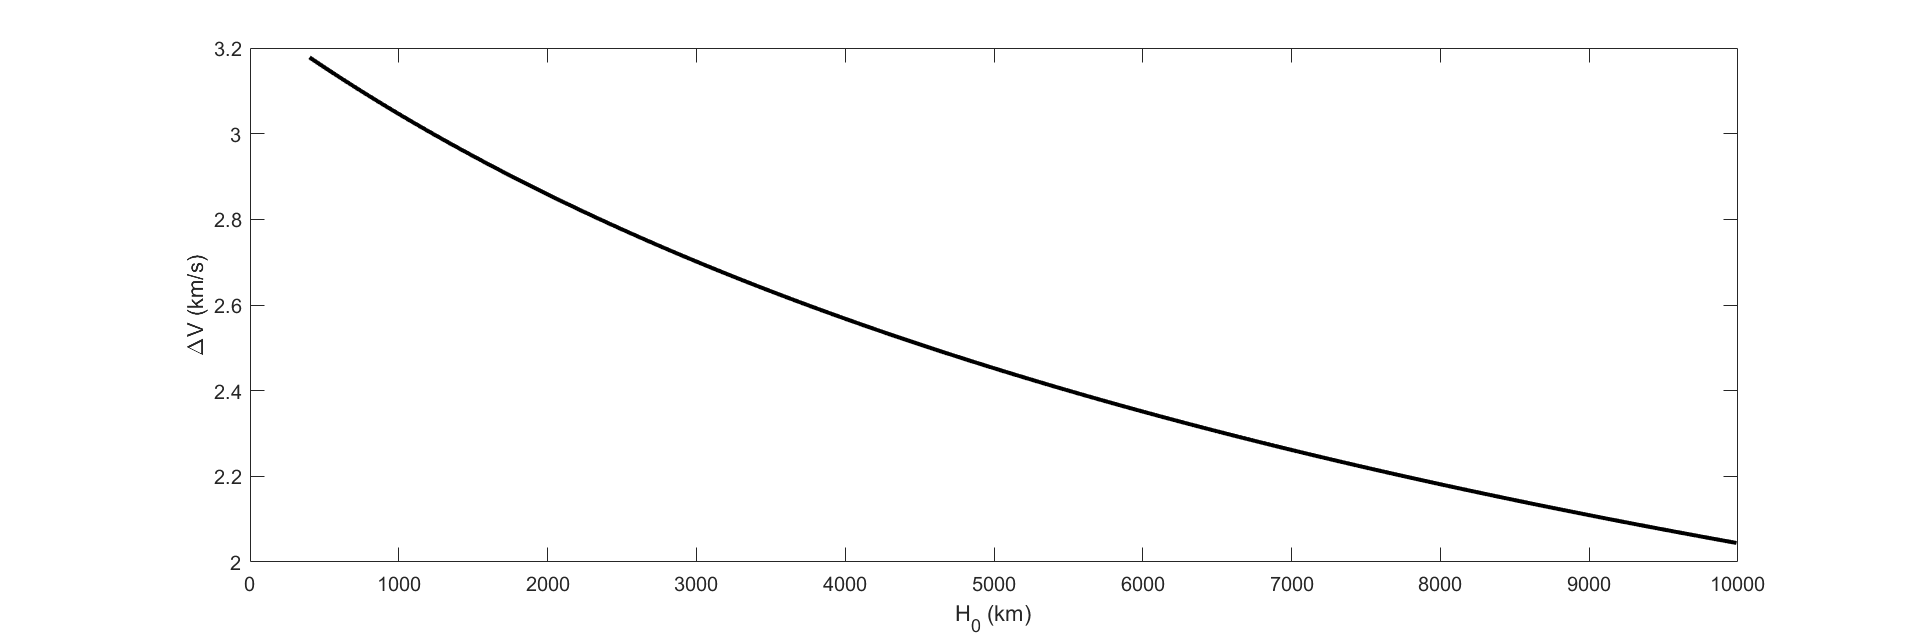
\includegraphics[width=\textwidth]{1a.png}
	\caption{$\Delta V$ vs $H_0$}
	\label{fig:1a}
\end{figure}


\subsection{Elliptic orbit}

\begin{figure}[H]
	\centering
		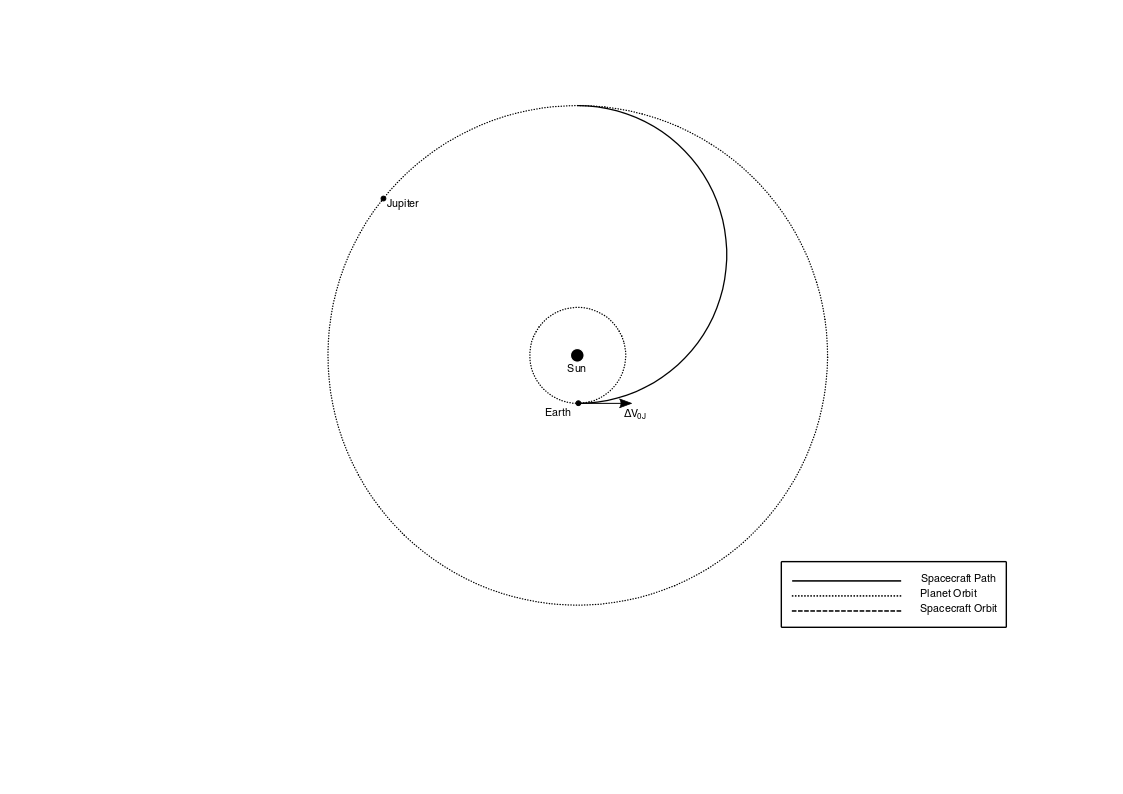
\includegraphics[width=\textwidth]{directa.png}
	\caption{Earth to Jupiter with one $\Delta V$}
	\label{fig:direct}
\end{figure}


The objective here is, again, escaping the Earth and orbit the Sun with an apoapsis radius equal to Jupiter's orbital radius ($r_a = d_{SJ}$). This time, however, just one thrust will be applied.

To do so, the spacecraft has to escape the Earth following a hyperbolic path, and enter, in consequence, an elliptical orbit around the Sun. The periapsis of this orbit will be at the point where the thrust is given, as shown in~\fref{fig:direct}

According to the conservation of energy, mechanical energy must remain constant. Therefore, the energy at the periapsis (where thrust maneuver is performed) is the same as the kinetic energy caused by the speed excess with respect to Earth ($V_\infty$). Thus, equation~\ref{eq:energy} is found by adding potential and kinetic in orbit energy of the spacecraft and equaling that to kinetic energy at infinity.

\begin{equation}\label{eq:energy}
E=\frac{\mu_{E}}{R_E + H_0} + \frac{(V_s + \Delta V_{0J})^2}{2}=\frac{(V_{\infty})^2}{2}
\end{equation}

As obtained $V_\infty$ is refered to Earth, the  orbital speed of the vehicle around the Sun will be calculated ($V_e$) by adding $V_\infty$ to Earth's orbital speed.
$\Delta V_{0J}$ is found by making $V_e$ equal to the vehicle's speed at an orbit around the Sun with $r_a = d_{SJ}$.

\begin{equation}\label{eq:thrust22}
\Delta V=\sqrt{\left(\sqrt{\mu_{Sun}\left(\frac{2}{d_{SE}}-\frac{1}{a}\right)}-\sqrt{\frac{\mu_{Sun}}{d_{SE}}}\right)^2+\frac{2\mu_E}{R_E+H_0}}-\sqrt{\frac{\mu_E}{R_E+H_0}}
\end{equation}
\paragraph{}
Equation~\ref{eq:thrust22} shows that $\Delta V$ depends on $H_0$, as previously deduced in \ref{sec:scape_maneuver}.

\begin{figure}[H]
	\centering
		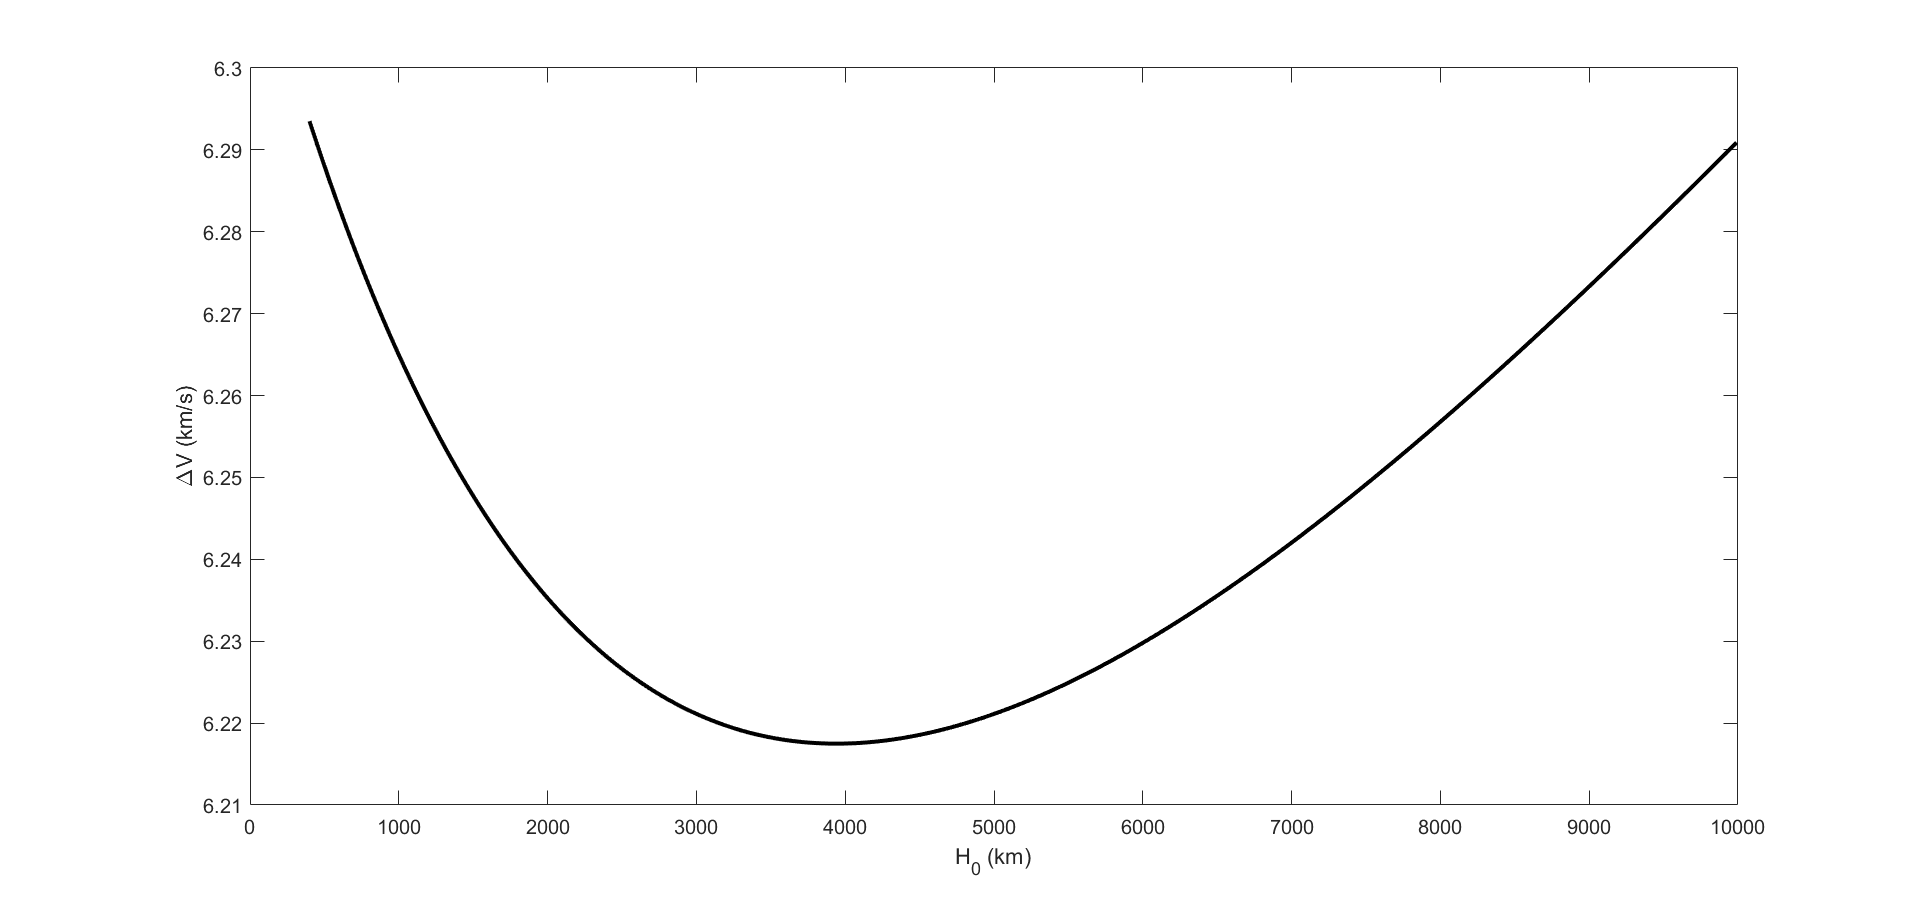
\includegraphics[width=\textwidth]{1b.png}
	\caption{$\Delta V$ vs $H_0$}
	\label{fig:1b}
\end{figure}

%%Figure 4
\subsubsection{Minimum $H_0$}
Thrust $\Delta V_{0J}$ is minimum when $H_0$ equals 3939 km (\fref{fig:1b}).From \fref{fig:1a} can be deduced that minimum $H_0$ of a parabolic scape path is at infinity.

\subsection{Direct transfer maneuver}

\begin{figure}[H]
	\centering
		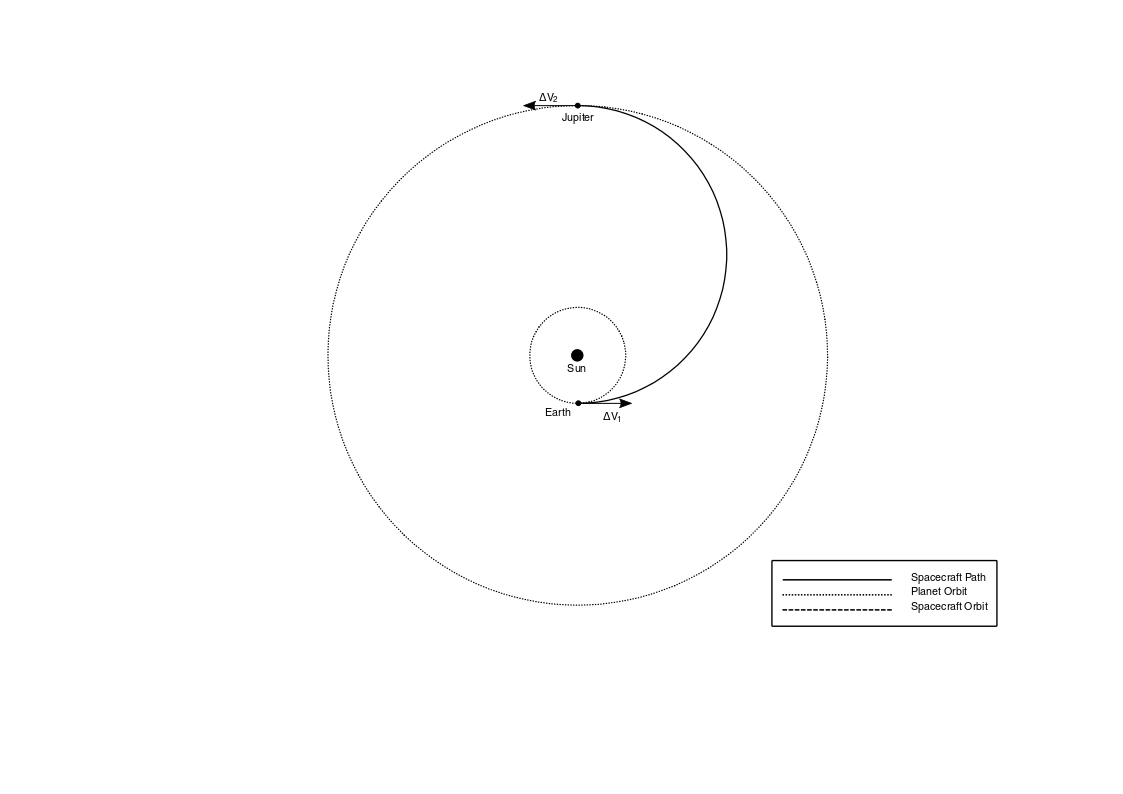
\includegraphics[width=\textwidth]{Hohman.png}
	\caption{Hohmann transfer maneuver $\Delta V$}
	\label{fig:Hohmann}
\end{figure}

In this part, the direct transfer maneuver from Earth to Jupiter will be developed. The main characteristic of this orbital maneuver is that the space vehicle traces a half elliptical orbit; in this case, with Jupiter orbital radius as apoapsis radius and Earth orbital radius as periapsis radius.To perform this Hohmann direct transfer maneuver two $\Delta V$ are needed. As seen in the figure above.  

The first $\Delta V$, ($\Delta V_1$) allows the vehicle to escape the orbit around the Earth, and places it in the transfer ellipse, with just one velocity impulse, as done in~\ref{sec:scape_maneuver}, using equation~\ref{eq:thrust22}. 

The second $\Delta V$, ($\Delta V_2$), applied in the ellipse apogee, will be the velocity that the vehicle has orbiting Jupiter minus the current velocity of the vehicle (velocity in the apogee of its elliptical orbit).

$$\Delta V_2 = \sqrt{\frac{\mu_{Sun}}{d_{SJ}}}-
\sqrt{2\mu_{Sun}\left(\frac{1}{d_{SJ}}-\frac{1}{2a}\right)}$$
  
The results are shown below:

\begin{itemize}

\item First impulse:

\begin{align*}
\Delta V_1&=\sqrt{\left(\sqrt{\left(\frac{2.654\times10^{11}}{1.5\times10^8}-\frac{1.327\times10^{11}}{4.643\times10^{8}}\right)}-\sqrt{\frac{1.327\times10^{11}}{1.5\times10^{8}}}\right)^2+\frac{7.972\times10^5}{6370+3939}}\\
&\quad-\sqrt{\frac{3.986\times10^5}{6370+3939}}
\end{align*}
$$\Delta V_1= 6.208 km/s $$

\item Second impulse:
$$\Delta V_2 = \sqrt{\frac{1.327\times10^{11}}{7.785\times10^8}}-
\sqrt{2\times1.327\times10^{11}\left(\frac{1}{{7.785\times10^{8}}}-\frac{1}{2\times 4.643\times10^{8}}\right)}$$

$$\Delta{V_2}= 5.633 km/s$$
\end{itemize}
The total velocity increment needed to perform the direct Hohmann maneuver can be obtained by adding both velocity increments.


\subsection{Insertion maneuver}

At this point, the vehicle has an orbital radius equal to Jupiter's orbital radius. The next step is to make the vehicle orbit Jupiter and put it into an orbit that has the same orbital radius than Jupiter's natural satellite Europa. 


The velocity of the vehicle at the apoapsis of its elliptical transfer orbit between the Earth and Jupiter:

 $$u_{a}=\sqrt{\mu_{Sun}\Big(\frac{2}{d_{SJ}}-\frac{1}{a}\Big)}=\sqrt{1.327\times10^{11}\Big(\frac{2}{7.785\times10^{8}}-\frac{1}{4.643\times10^{8}}\Big)} = 7.423 km/s$$
 
 
 By means of the law of conservation of energy, it is stated the energy of the vehicle  (with respect to Jupiter) has to remain the same before and after the gravitational influence. 
 
                $$\frac{(v_{\infty})^2}{2}=\frac{(v_{p})^2}{2}-\frac{\mu_{Jupiter}}{d_{Jupiter-Europa}}$$
                
                Where:
                $$v_{\infty}=u_{a-Jupiter}-u_{Jupiter}$$
                $$v_p=\Delta{V}+v_{vehicle}$$
                
 Thus: $$\frac{(u_{a-Jupiter}-u_{Jupiter})^2}{2}=\frac{(\Delta{V}+v_{vehicle})^2}{2}-\frac{\mu_{Jupiter}}{d_{Jupiter-Europa}}$$
 
 After operating:
               
               $$\Delta{V}=\sqrt{\Big(u_{a-Jupiter}-u_{Jupiter}\Big)^2+\frac{2\mu_{Jupiter}}{d_{Jupiter-Europa}}}-v_{vehicle}$$

\begin{equation}\label{eq:insertion}
\Delta{V}=\sqrt{\Big(u_{a-Jupiter}-\sqrt{\frac{\mu_{Sun}}{d_{SJ}}}\Big)^2+\frac{2\mu_{Jupiter}}{d_{Jupiter-Europa}}}-\sqrt{\frac{\mu_{Jupiter}}{d_{Jupiter-Europa}}}
\end{equation}

          
          {$$\Delta{V}=\sqrt{\Bigg(7.423 - \sqrt{\frac{1.327\times10^{11}}{7.785\times10^{8}}}\Bigg)^2+\frac{2\times1.267\times10^{8}}{6.71\times10^{5}}}-\sqrt{\frac{1.267\times10^{8}}{6.71\times10^{5}}}$$}
          
          $$\Delta{V} = 6.492 km/s$$
         
The needed time for the vehicle to arrive to Jupiter and orbit it can be estimated by means of Kepler's third law, which gives the period of the elliptical orbit. As only half of the elliptical orbit is traversed, the actual time will be half of the obtained period.

\begin{equation}
\frac{T^2}{a^3}=\frac{4\pi^2}{\mu}
\end{equation}

In this case, the time is:

$$t=\frac{1}{2}\sqrt{\frac{4\pi^2a^3}{\mu_{Sun}}}=\pi\sqrt{\frac{\left(d_{SE}+d_{SJ}\right)^3}{\mu_{Sun}}}$$
\begin{itemize}

\item The required time to execute the maneuver:
$$t=\pi\sqrt{\frac{\left(4.643\times10^{8}\right)^3}{1.327\times10^{11}}}= 2.74 years $$

This equation is just an approximation. Note that the needed time to perfom the insertion maneuver is neglected. It is only taken into account the time needed to perfom the Hohmann transfer shown in the previous section, eventhough the actual time would be obtained by adding both times. A more precise calculation is developed as a bonus part.

\end{itemize}


\subsection{Natural gravity assist} 
\begin{figure}[H]
	\centering
		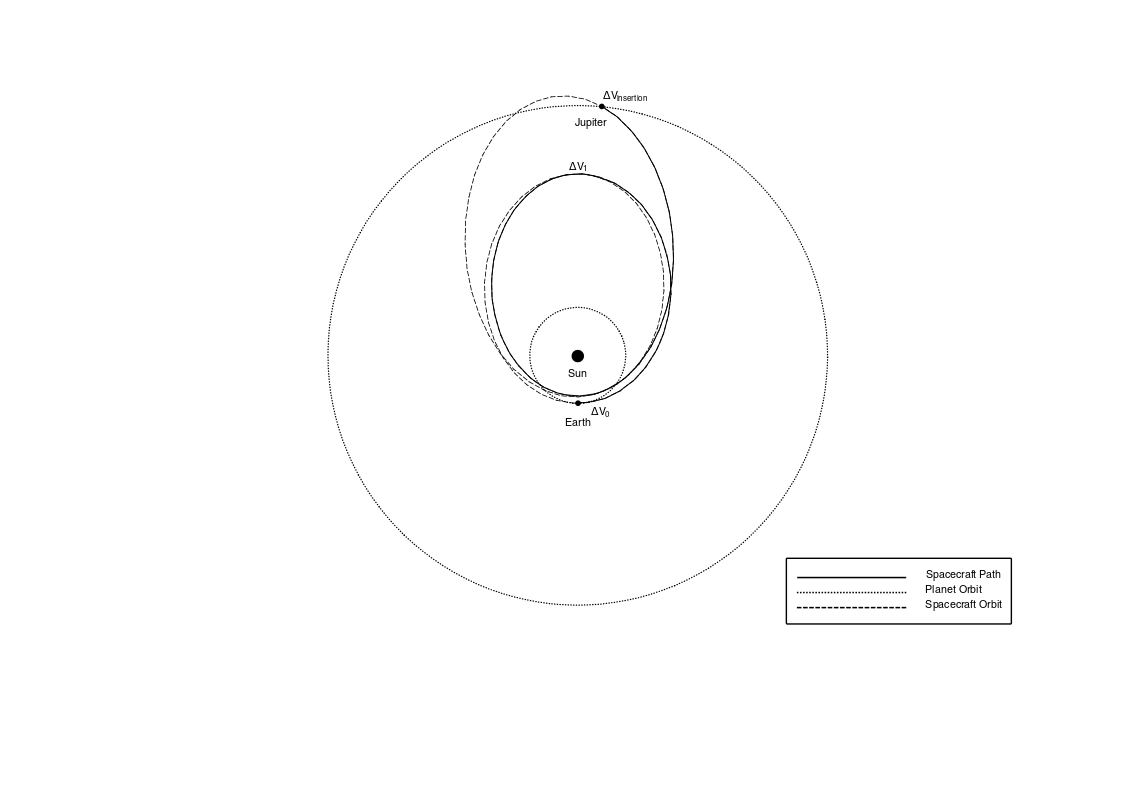
\includegraphics[width=\textwidth]{flyby.png}
	\caption{Earth to Jupiter for $H_\pi = 450km$}
	\label{fig:flybytrim}
\end{figure}

This maneuver consists of applying three speed increments. The first one is needed to escape the Earth, the second one to modify the trajectory and encounter the Earth to perform the gravitational assist maneuver and the last one, it will be a velocity increment to enter the orbit of Jupiter.

To begin, it is necessary to calculate satelite's scape speed with respect to the Sun ($u_{1p}$).
The spacecraft leaves the Earth with a hyperbolic orbit, that means that it will have an elliptical orbit around the sun. Let $v_s$ be the orbital speed of the satellite, $V_\infty$ is calculated by conservation of energy.

\begin{equation*}
V_\infty = \sqrt{(v_s + \Delta V_0)^2 - \frac{2 \mu_E}{R_E + H_0}}
\end{equation*}

Therefore, $u_{1p}$ is given by
\begin{equation*}
u_{1p} = V_\infty + u_E
\end{equation*}

Next, it is necessary to calculate the parameters of this ellipse, in this case the eccentricity and the apoapsis radius.

\begin{equation*}
e_1 = \frac{h_1^2}{\mu d_{SE}} - 1 
\end{equation*}

\begin{equation*}
d_{1a} = \frac{h_1^2}{\mu (1 - e)}
\end{equation*}

Knowing that $h_1=d_{SE}u_{1p}$.
Then, velocity at apoapsis $u_{1a}$ is calculated by means of the law of conservation of angular momentum.

At the apoapsis the brake thrust is applied, and the new speed will be $u_{2a} = u_{1a} + \Delta V_1$. Again, the parameters of the ellipse are needed.

\begin{equation*}
e_2 = 1 - \frac{h_2^2}{\mu d_{1a}}  
\end{equation*}

\begin{equation*}
d_{2p} = \frac{h_2^2}{\mu(1 + e)}
\end{equation*}

u1This new orbit intersects the Earth's orbit at an angle $\theta_i$, which is the true anomaly of the orbit at the intersection point, where the spacecraft's orbital radius equals to the Earth orbital radius.

\begin{equation}
\theta_i = \arccos\left[\frac{a_2(1-e_2^2)- d_{SE}}{e_2d_{SE}}\right]
\end{equation}

The last equation has two different solutions (two different angles), but there will be just one correct answer, the one that gives a tangent velocity at that point. 

\begin{equation}
\vec{u_s}^- = \sqrt{\frac{\mu_S}{a2(1 - e_2^2)}}
\left(
\begin{array}{c}
-\sin\theta_i\\
e_2 + \cos\theta_i
\end{array}
\right)
\end{equation}

Earth's speed vector is
\begin{equation*}
\vec{u_E} = \sqrt{\frac{\mu}{d_{SE}}}
\left(
\begin{array}{c}
-\sin\theta_i\\
\cos\theta_i
\end{array}
\right)
\end{equation*}

Therefore, the speed of the spacecraft with respect to the Earth before the assist is:
\begin{equation*}
\vec{v}^-_\infty = \vec{u_s}^- - \vec{u_E}
\end{equation*}

And the speed after the assist with respect to the Sun will be
\begin{equation}\label{eq:uplus}
\vec{u_s}^+ = \vec{v}^+_\infty + \vec{u_E}
\end{equation}

As the spacecraft describes a hyperbolic path around the Earth, if the law of conservation of the energy is applied, the result is $v_\infty^- = v_\infty^+$. Speed modulus with respect to the Earth is the same before and after the maneuver, but the direction of the vector changes.

\begin{equation}
\vec{v}^+_\infty = R(\delta)\vec{v}^-_\infty
\end{equation}

The rotation matrix is

\begin{equation*}
R(\delta) = \left(
\begin{array}{cc}
\cos\delta & -\sin\delta \\
\sin\delta & \cos\delta
\end{array}
\right)
\end{equation*}

where $\delta$ is the angle between the speed vector at the entry and exit.

\begin{equation*}
\delta = 2\left(\pi - \arcsin\left(\frac{1}{e_{hyp}}\right)\right)
\end{equation*}

and 
\begin{equation*}
e_{hyp} = 1 + \frac{r_\pi v_\infty^2}{\mu_E}
\end{equation*}

It can be seen that the speed after the fly-by maneuver (given by \eqref{eq:uplus})  is a function of $H_\pi$, as $r_\pi = R_E + H_\pi$.

Now, the parameters of the approach orbit are required. Apoapsis radius can be calculated by
\begin{equation}\label{eq:d3a}
d_3a = \frac{h_3^2}{\mu(1-e)}
\end{equation}

where the eccentricity is given by

\begin{equation}\label{eq:e_ellipse_urmu}
\vec{e} = \frac{\left(\vnorm{u}^2 - \frac{\mu}{\vnorm{r}}\right) \vec{r} - \left(\vec{r}\cdot\vec{u}\right) \vec{u}}{\mu}
\end{equation}

By operating \eqref{eq:e_ellipse_urmu} and substituting in \eqref{eq:d3a} the value is calculated.

Finally, it is necessary to calculate the total thrust.

\begin{equation*}
\Delta V_T = \Delta V_0 + \Delta V_1 + \Delta V_{insertion}
\end{equation*}

Where $\Delta V_{insertion}$ is calculated with \eqref{eq:insertion}. 

To minimize this non-linear multi-variable function it would be necessary to use numerical methods. For example, a genetic algorithm could be implemented.

\begin{figure}[H]
	\centering
		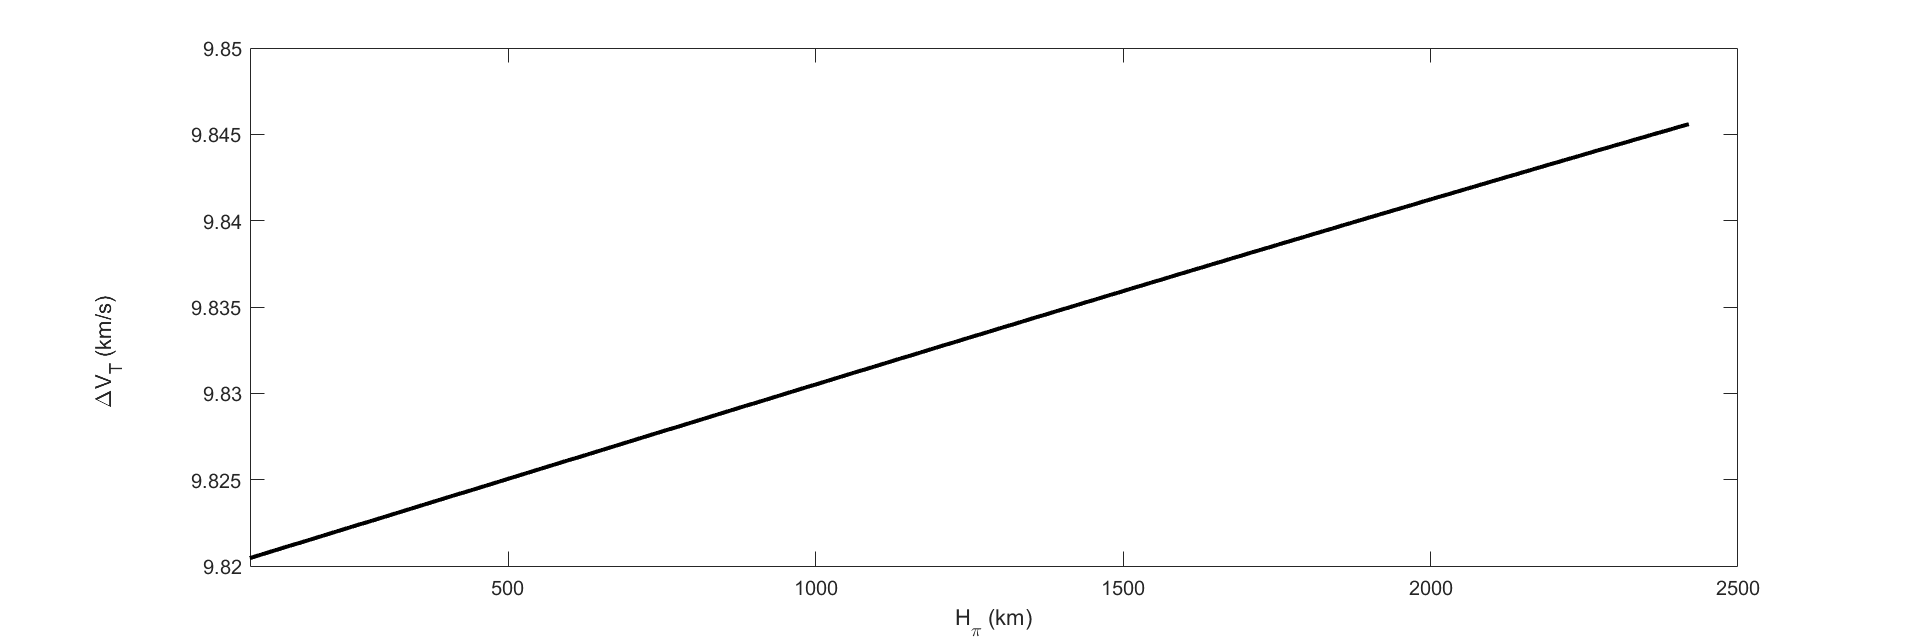
\includegraphics[width=\textwidth]{untitled.png}
	\caption{$\Delta V_T$ vs $H_\pi$}
	\label{fig:2b}
\end{figure}

% REGULA FALSI 


\subsection{Jupiter travel's Time}
Kepler's equation, wich relates various geometric properties of the orbit of a body subject to a central force, is defined by:
\begin{equation}\label{eq:Kepler}
M=E-esinE
\end{equation}
where $E$ is the eccentric anomaly,
$M$ is the mean anomaly and $e$ is the eccentricity of the orbit:
\begin{equation*}
e=\frac{r_pv_p^2}{\mu}-1
\end{equation*}
\begin{equation*}
E=\arccos\left(\frac{e+cos\theta}{1+ecos\theta}\right)
\end{equation*}
\\
Knowing that $M$ depends of the travel time, it can be isolated:
\begin{equation}\label{eq:m_anomaly}
M=\sqrt{\frac{\mu}{a^3}}(t-\tau)
\end{equation}
where 
\begin{equation*}
a=\frac{r_p^2v_p^2}{\mu (1-e)}
\end{equation*}
\\
and $\tau$ is the time at which the body is at the periapsis. From~\eqref{eq:Kepler} and~\eqref{eq:m_anomaly}:

\begin{equation*}\label{eq:130}
E-esinE=\sqrt[]{\frac{\mu}{a^3}}(t-\tau)
\end{equation*}
\\
Setting $\tau=0$ 
\begin{equation}\label{eq:temps}
t=(E-esinE)\sqrt{\frac{a^3}{\mu}}
\end{equation}

To calculate the travel time from the last section the expresion \eqref{eq:temps} will be used. 
It can be divided in three parts: travel time to reach the apoapsis of the first orbit ($t_1$), time to travel from the apoapsis back to Earth ($t_2$), and time from Earth to Jupiter after the gravity assist ($t_3$). Gravity assist and insertion maneuvers' time will be considered negligible.
\begin{equation*}
t_{T}=t_{1}+t_{2}+t_{3}
\end{equation*}
$t_{1}$ is easily calculated directly aplying the formula for $\theta=\pi$:
\begin{equation*}
t_1=(E_1-e_1sinE_1)\sqrt{\frac{a_1^3}{\mu_S}} % CALCULAR
\end{equation*}

$t_{2}$ can be calculated by adding the time needed to reach the Earth from the periapsis and the time needed to reach the periapsis from the apoapsis. Due to the symetry of the orbit, the latter one is equal to the time to needed to reach the apoapsis from the periapsis.
\begin{equation*}
t_2=(E_{2;\theta=\pi}-e_2sinE_{2;\theta=\pi}+E_{2;\theta=\theta_{int}}-e_2sinE_{2;\theta=\theta_{int}})\sqrt{\frac{a_2^3}{\mu_S}} % CALCULAR --> ANGLEEE
\end{equation*}

Lastly, $t_3$ is calculated by substracting the time from the periapsis to the intersection point from the time from the periapsis to Jupiter in Jupiter's approach orbit. 
\begin{equation*}
t_3=(E_{3;\theta=\theta_J}-e_3sinE_{3;\theta_J}-(E_{3;\theta=\theta_{int}}-e_3sinE_{3;\theta=\theta_{int}}))\sqrt{\frac{a_3^3}{\mu_S}} % CALCULAR --> ANGLEEE (Respecte a la nova òrbita)
\end{equation*}

That way it can be seen that $\tau=0$ and there is no need to calculate it. \\

$\theta_J$ is the angle of intersection with Jupiter. This can be done with:

\begin{equation*}
\cos{\theta} = \frac{\vec{e}\cdot\vec{r}}{\vnorm{e} \vnorm{r}}
\end{equation*}
% ESQUEMA ÒRBITES 1, 2, 3

Total travel time to reach Jupiter:
\begin{equation*}
t_T = 1.03 + 1.08 + 2.72 = 4.83 years
\end{equation*}

\nocite{franchini2008introduccion}
\nocite{curtis2013orbital}
\section{Schemes}\label{sec:schemes}
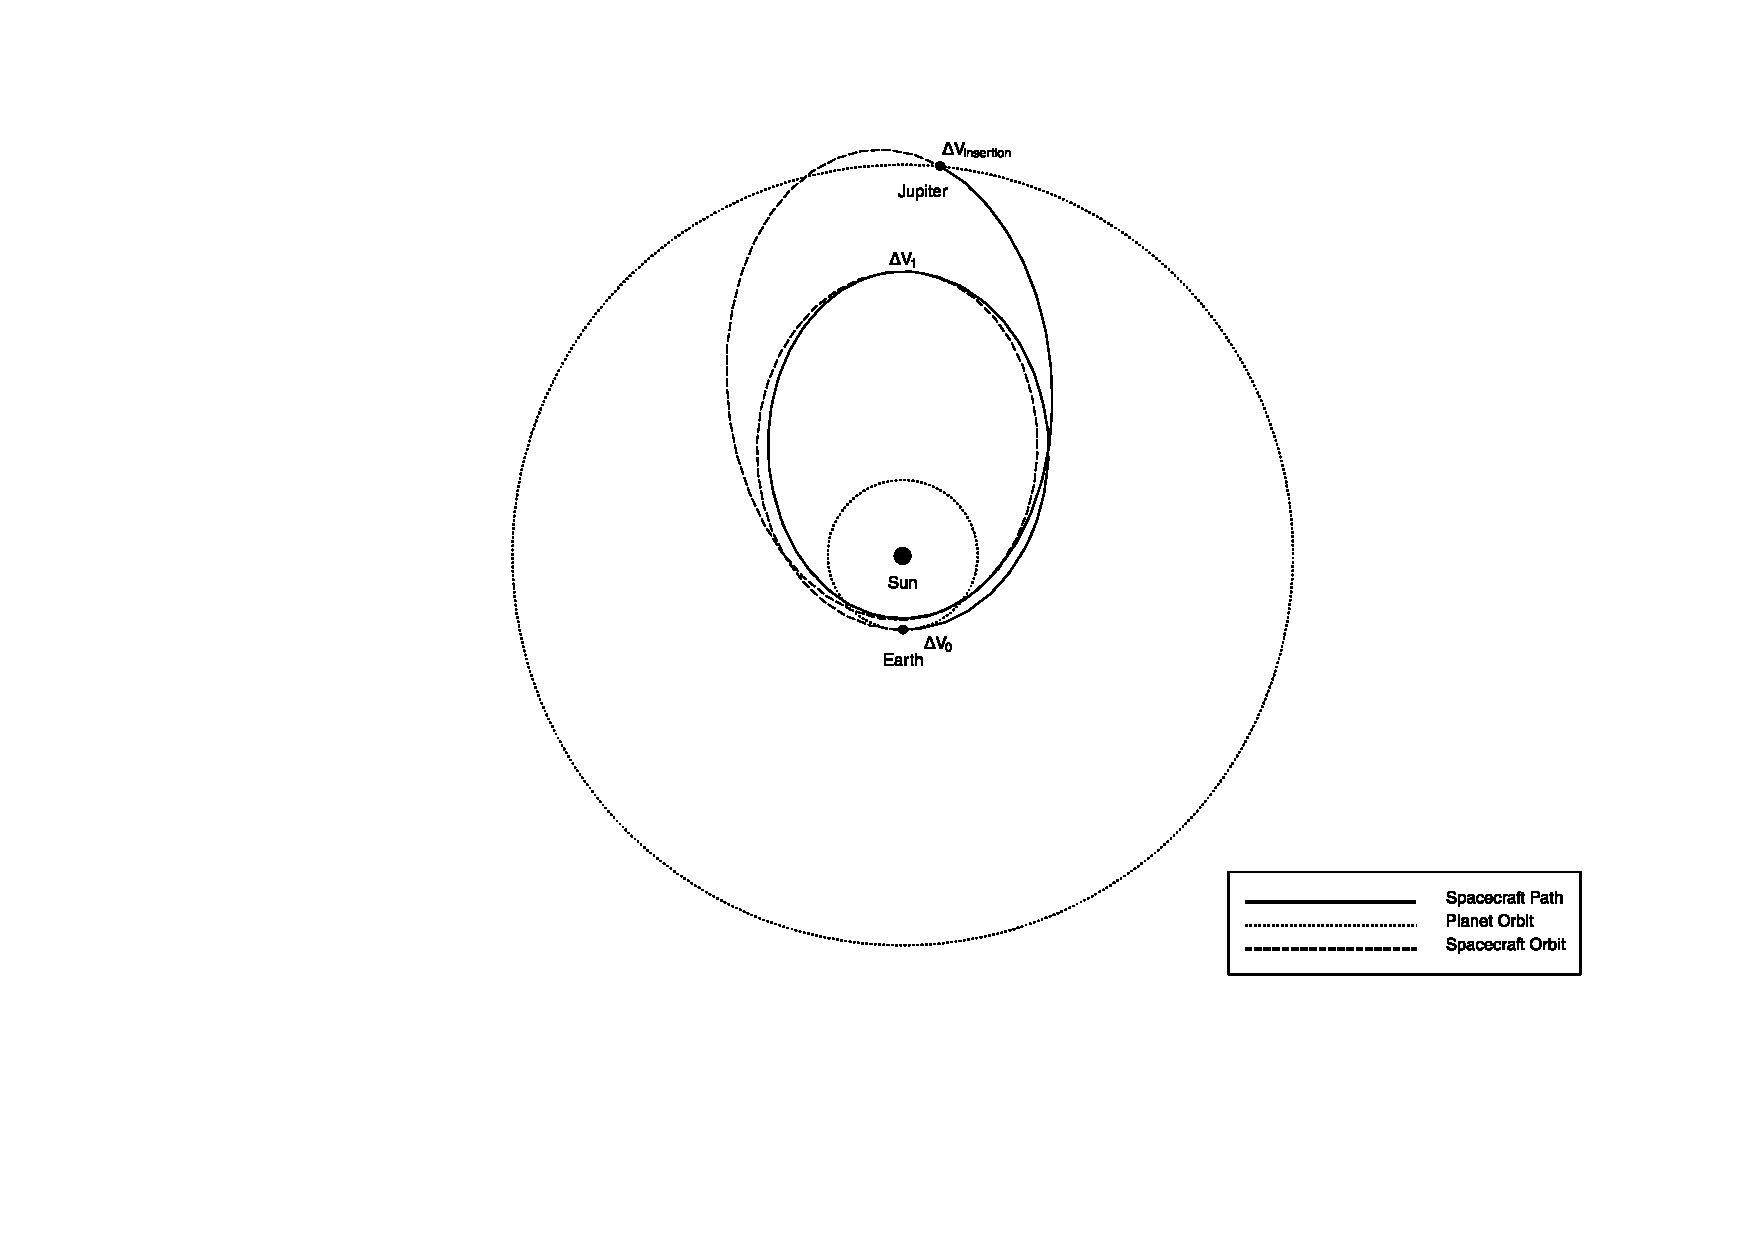
\includepdf{flby.pdf}

\section{Conclusions}\label{sec:conclusions}

Throughout the assignment it can be noted that it is more efficient to exit the Earth's gravitational influence by means of an hyperbolic trajectory rather than a parabollic one. That is because in the latter, a second speed increment is needed, hence making the total speed increment larger.

Then, to reach Jupiter, it can be shown that, eventhough it takes much longer to reach Jupiter with a fly-by maneuver, both the initial speed increment and the needed one to describe an orbit around Jupiter with the same orbital radius than Europa, are significantly lower. When it comes to space missions, saving fuel is prioritised, so it can be concluded that the best way to reach Jupiter will be by means of the fly-by maneuver.  

During the document, it is assumed that $r_{SOI} = 0$ for all celestial bodies, so the vechicle is only under the influence of just one gravitational field at a point. Besides, it has not been taken into consideration the event of possible collisions between celestial bodies.

All in all, this is a preliminary study that cannot be used to describe the exact trajectory that the vehicle has to follow -it would be affected by the gravitational fields of other celestial bodies apart from the Sun, the Earth and Jupiter- but it presents a good first approximation and estimation of the initial velocity increment that is needed to reach such destination. 


\printbibliography[heading=bibintoc]


\appendix
\section{Source code}

\lstset{%
tabsize=2,
postbreak=\mbox{\textcolor{red}{$\hookrightarrow$}\space},
columns=fullflexible,
breaklines=true,
breakatwhitespace=true,
literate={::}{}{0\discretionary{::}{}{::}}% line-break at ::
         {->}{}{0\discretionary{->}{}{->}}% line-break at ->
         {<<}{}{0\discretionary{<<}{}{<<}}% line-break at <<
         {,}{}{0\discretionary{,}{}{,}}% line-break at ,
         {-}{}{0\discretionary{-}{}{-}}% line-break at -
}
\lstinputlisting{codi.cpp}[language=C++]
% \begin{lstlisting}[language=C++]
% /*
%  * Your code goes here or instead you can use the command:
%  * \lstinputlisting{solution.cpp}[language=C++]
%  * and comment the \begin and \end lstlisting
%  * where solution.cpp is the name of the file that contains your code.
%  */

% double a_ellipse(double mu, double u, double r){
% 	return mu*r / (2.0*mu - u*u * r);
% } 

% cout << "up0*up0 - 2*muT/(H+6371.0e3) = " << (up0*up0 - 2.0*muT/(H+6371.0e3)) << endl;

% \end{lstlisting}


%\lstinputlisting[language=C++]{solution.cpp}


% \newpage

{\color{red}\textbf{Delete the following pages on the final report! If you use some of the equations explain them somewhere in your text.}}

\section*{Form equations}

\subsection*{Ellipse}

\eref{eq:e_ellipse_urmu} defines the eccentricity of an elliptic orbit around an object of gravitational parameter $\mu$, knowing the velocity $\vec{u}$ at a radius $\vnorm{r}$.

\begin{equation}\label{eq:e_ellipse_urmu}
\vec{e} = \frac{\left(\vnorm{u}^2 - \frac{\mu}{\vnorm{r}}\right) \vec{r} - \left(\vec{r}\cdot\vec{u}\right) \vec{u}}{\mu}
\end{equation}

The true anomaly $\theta$ is defined by \eref{eq:theta_er}, where $\vec{e}$ is the eccentricity, as defined in \eref{eq:e_ellipse_urmu}, and $\vec{r}$ is the radius.

\begin{equation}\label{eq:theta_er}
\cos{\theta} = \frac{\vec{e}\cdot\vec{r}}{\vnorm{e} \vnorm{r}}
\end{equation}

\section*{Notes}

Read the following commentaries and follow them:

\begin{itemize}
\item The assignment consists on completing the report. This is to complete the existing sections and to write the empty ones. A general structure of the report is proposed but you can change the empty sections if you like. Just keep it organized. Do not include the sections \textit{Form equations} and \textit{Notes} in the final document.

\item Replace the group number, currently indicated as 'AB' for your group number; and replace the names of the authors (your names) for the names of the teachers.

\item Detail the formulation used for each point of the report, but avoid repeating it. Instead make references to the sections where they are detailed the first time and indicate the values that are used. So try to define general formulation of orbital mechanics and apply it to answer the points of the report. A good strategy could be to create a section with the formulation needed across the report and refer to it in the results sections.

\item Do not forget the units of any magnitude in the report, except if they are dimensionless. The units must be indicated also in the graphics.

\item Present the graphics with interplanetary distances in astronomical units.

\item Present the graphics in black with different styles of lines and/or points.

\item Cite the sources you use. It is preferable to use references to books than digital content. If you use references to digital content, include the year and month on the cite. You can add the description of the cite in \textit{myrefs.bib} and use the command \textit{autocite} in the text. Example \autocite{franchini2008introduccion}.

\item The script or code used to solve the problem must be delivered with the report. It has to be well organized and with commentaries explaining which point is being solved, and the major steps of each solution. We recommend to use C/C++, Python, Octave or Matlab; but fell free to use other languages as long as you indicate which one is being used.

\item The grade you can achieve is not proportional to the number of pages. Actually it can be the opposite, if you talk too much you can say things that are not correct. So be concise and accurate.
\end{itemize}

Example to insert an image, the \fref{fig:etseiatlow} shows bla bla.

% 0.7 is the size respect to \linewidth

\begin{figure}[htb]
  \centering
   
\includegraphics[width=0.7\linewidth]{etseiatlow}
   \caption{Here goes the caption text.}
   \label{fig:etseiatlow2}
\end{figure}

\imatge{etseiatlow}{Here goes the caption text.}{0.7}

Another way to do it, the \fref{fig:etseiatlow2} shows bla bla.



%\subsection*{Hyperbola}





\end{document}